\subsection{Translations}
\UPSTIdefinition[Mouvement de Translation]{Un solide est en mouvement de translation lorsqu'un
segment quelconque de ce solide reste parallèle à lui-même au cours du déplacement.}

%\UPSTIremarque{
Cela revient à dire que lorsqu'un solide est en translation, toutes les photos prises de cet objet au cours du temps seraient identiques
%}

\subsubsection{Translation rectiligne}
\UPSTIexemple[Une voiture en ligne droite]{
  La voiture de la \UPSTIfig{fig:rectiligne} est translation rectiligne.
  \begin{figure}[!ht]
    \centering
    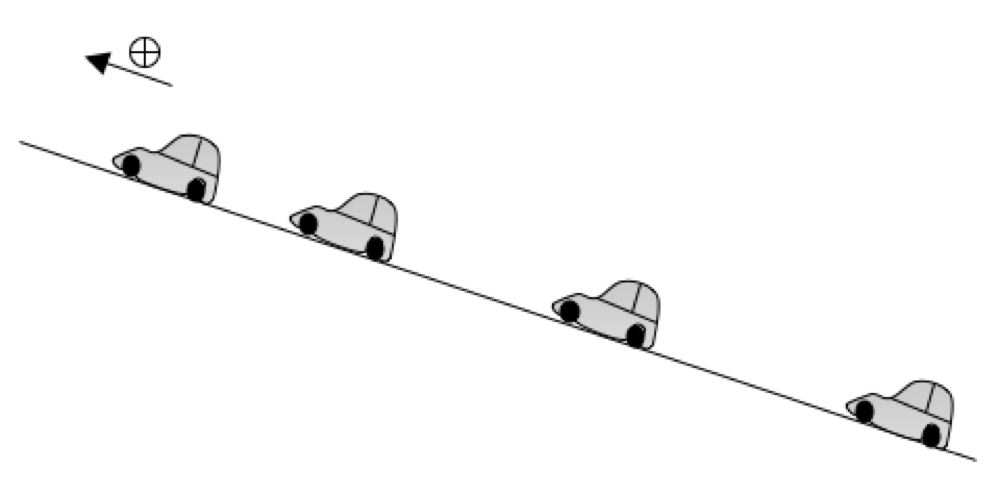
\includegraphics[width=.4\textwidth]{Src/Images/voiture_translation}
    \caption{Translation rectiligne}
    \label{fig:rectiligne}
  \end{figure}
}

\UPSTIaRetenir{Une translation est dite \textbf{rectiligne} lorsque les trajectoires des points du solides sont des \textbf{segments} (ou droites).}

\UPSTIaRetenir{La translation rectiligne uniforme désigne un mouvement de translation en \textbf{ligne droite} et à \textbf{vitesse constante}.}

\begin{UPSTIactivite}
  Soit une voiture en translation rectiligne uniforme de vitesse $v=\SI{15}{m/s}$.
  \UPSTIquestion{Calculer la distance parcourue en \SI{20}{min}}

  \UPSTIeleveOnly{\UPSTIpointilles}

   \begin{UPSTIcorrectionEnv}{

     On a $v=\SI{15}{m/s}$. On sait que $v=\frac{d}{\Delta t}$. On a donc $d=v\times\Delta t = 15 \times 20\times 60 = \SI{18000}{m} = \SI{18}{km}$ }
   \end{UPSTIcorrectionEnv}

  \UPSTIquestion{Que vaut l'accélération de cette voiture ?}

  \UPSTIeleveOnly{\UPSTIpointilles}
\begin{UPSTIcorrectionEnv}{

  La vitesse étant constante, l'accélération est nulle.}
\end{UPSTIcorrectionEnv}
\end{UPSTIactivite}


\subsubsection{Translation circulaire}
\UPSTIexemple[Une cabine de grande roue]{
  La cabine supendue à la grande roue de la \UPSTIfig{fig:circulaire} est translation circulaire.
  \begin{figure}[!ht]
    \centering
    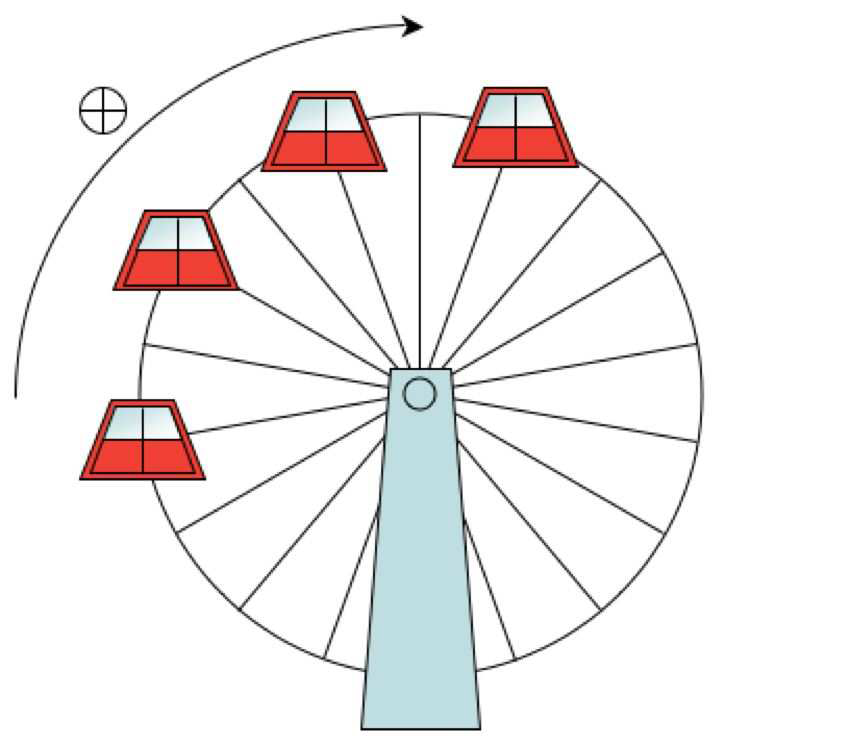
\includegraphics[width=.4\textwidth]{Src/Images/translation_circulaire_manege}
    \caption{Translation circulaire}
    \label{fig:circulaire}
  \end{figure}}
  \UPSTIaRetenir{Une translation est dite \textbf{circulaire} lorsque les trajectoires des points du solides sont des \textbf{cercles}.}

  \UPSTIattention{La grande roue est en rotation, c'est bien la \textbf{cabine} qui est en translation ciruclaire car elle se déplace sans tourner par rapport au sol}


\subsubsection{Translation curviligne}
\UPSTIexemple[Une cabine de téléphérique]{
  La cabine du téléphérique de la \UPSTIfig{fig:curviligne} est translation curviligne.
  \begin{figure}[h!t]
    \centering
    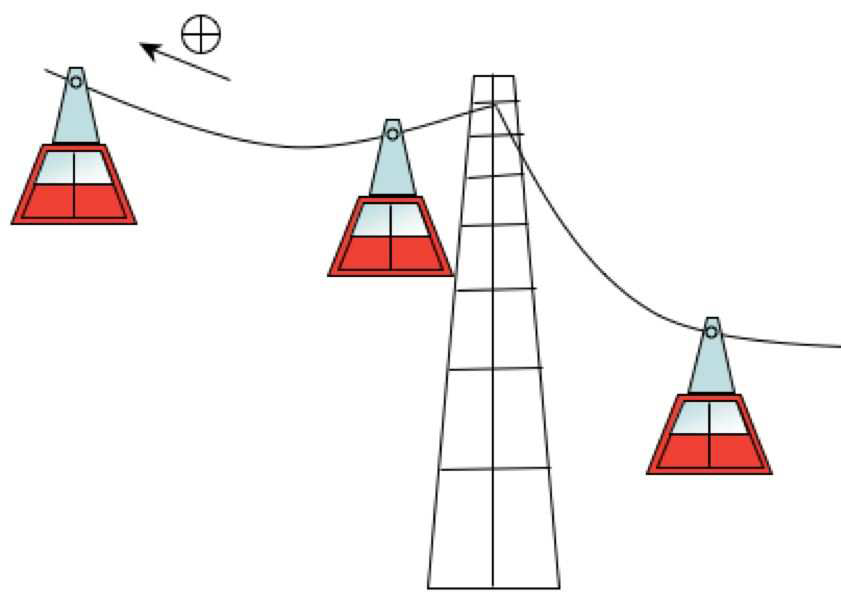
\includegraphics[width=.35\textwidth]{Src/Images/translation_curviligne_telesiege}
    \caption{Translation curviligne}
    \label{fig:curviligne}
  \end{figure}
}

\UPSTIaRetenir{Une translation est dite \textbf{curviligne} lorsque les trajectoires des points du solides sont des \textbf{courbe}. C'est à dire lorsqu'il s'agit d'une translation qui n'est ni rectiligne, ni circulaire.}

\subsection{Rotation}
\UPSTIexemple[Une bouteille de lait que l'on fait tourner]{
La bouteille de lait de la \UPSTIfig{fig:rotation} est en rotation.
\begin{figure}[h!t]
  \centering
  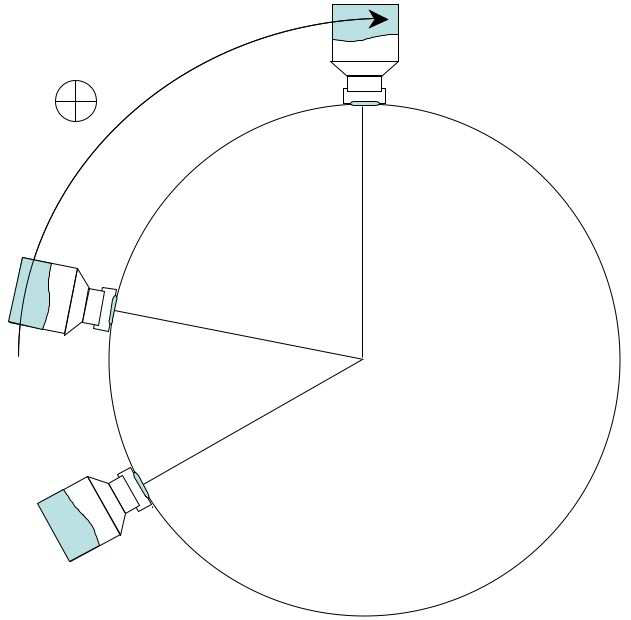
\includegraphics[width=.4\textwidth]{Src/Images/rotation_lait}
  \caption{Rotation}
  \label{fig:rotation}
\end{figure}
}
\UPSTIdefinition{Un solide est en mouvement de rotation lorsque tout point de ce solide reste à une distance fixe du centre de rotation. Cela veut dire que tous les points du solide se déplacent sur des cercles qui ont un même centre.}
